\documentclass{article}
\usepackage[utf8]{inputenc}
\usepackage{csquotes}
\usepackage{natbib}
\usepackage{graphicx}
\usepackage{float} 
\usepackage{epsfig}
\usepackage{siunitx}
\begin{document}
\begin{titlepage}
	\begin{center}
		\Huge\textbf{EE-568 }\\
		\vspace{0.5cm}
		\Huge\textbf{HW-1}\\
		\vspace{0.5cm}
		\Huge\textbf{Torque in a Variable Reluctance Machine}\\
		\vspace{0.5cm}
		
\includegraphics[scale=1]{E:/Github/EE568/HW1/Rapor/Figurler/odtulogo}\\
		
		
		\Large\textbf{Prepared by:}Hakan POLAT\\
		
		\Large\textbf{Submitted to:} Dr. Ozan KEYSAN\\
		\vspace{0.5cm}
		\Large\textbf{Electrical and Electronics Engineering Department}\\
		
		\large\textbf{ANKARA	}\\
		\large\textbf{05.03.2020}\\
		
		
		
	\end{center}
	
	

\end{titlepage}

\newpage
\section{Introduction}
In this report a variable reluctance machine is investigated both analytically and numerically. In the first part, the system parameters will be delivered. In the next part, an analytic derivation for the reluctance and inductance will be made for the machine under investigation. The torque produced under DC excitation will be derived and presented. Then additional methods for improving the analitic approach will be discussed.\\
In the next part, results for 2D finite element model of the machine will be presented. The analysis is done in ANSYS Maxwell environment. The core material is selected as laminated steel and the permeability is taken as linear. The flux densities for degrees 0,45 and 90 are plotted. The inductance, stored energy and torque is calculated using finite element analysis. The results are then compared to the analytical results and the differences are discussed. \\
In the final part, a non-linear core material is selected. The effect of core saturation is observed. The analysis performed in previous section is repeated. Again the analysis results are compared to the analytical model and the linear core material cases and discussed.

\section{System Parameters and Dimensions}
The variable reluctance machine under investigation is presented in Fig. \ref{fig:system}. The machine constist of three parts. The coil windings are used to generated flux. The core is used to direct the flux and torque generated on the rotational section. The coils are wound within 30~mmx10~mm rectangle, each airgap clearance is 0.5~mm, depth of the core is 20~mm, number of turns is 250 and the excitation current is 3A~DC.
\begin{figure}[h!]
	\centering
	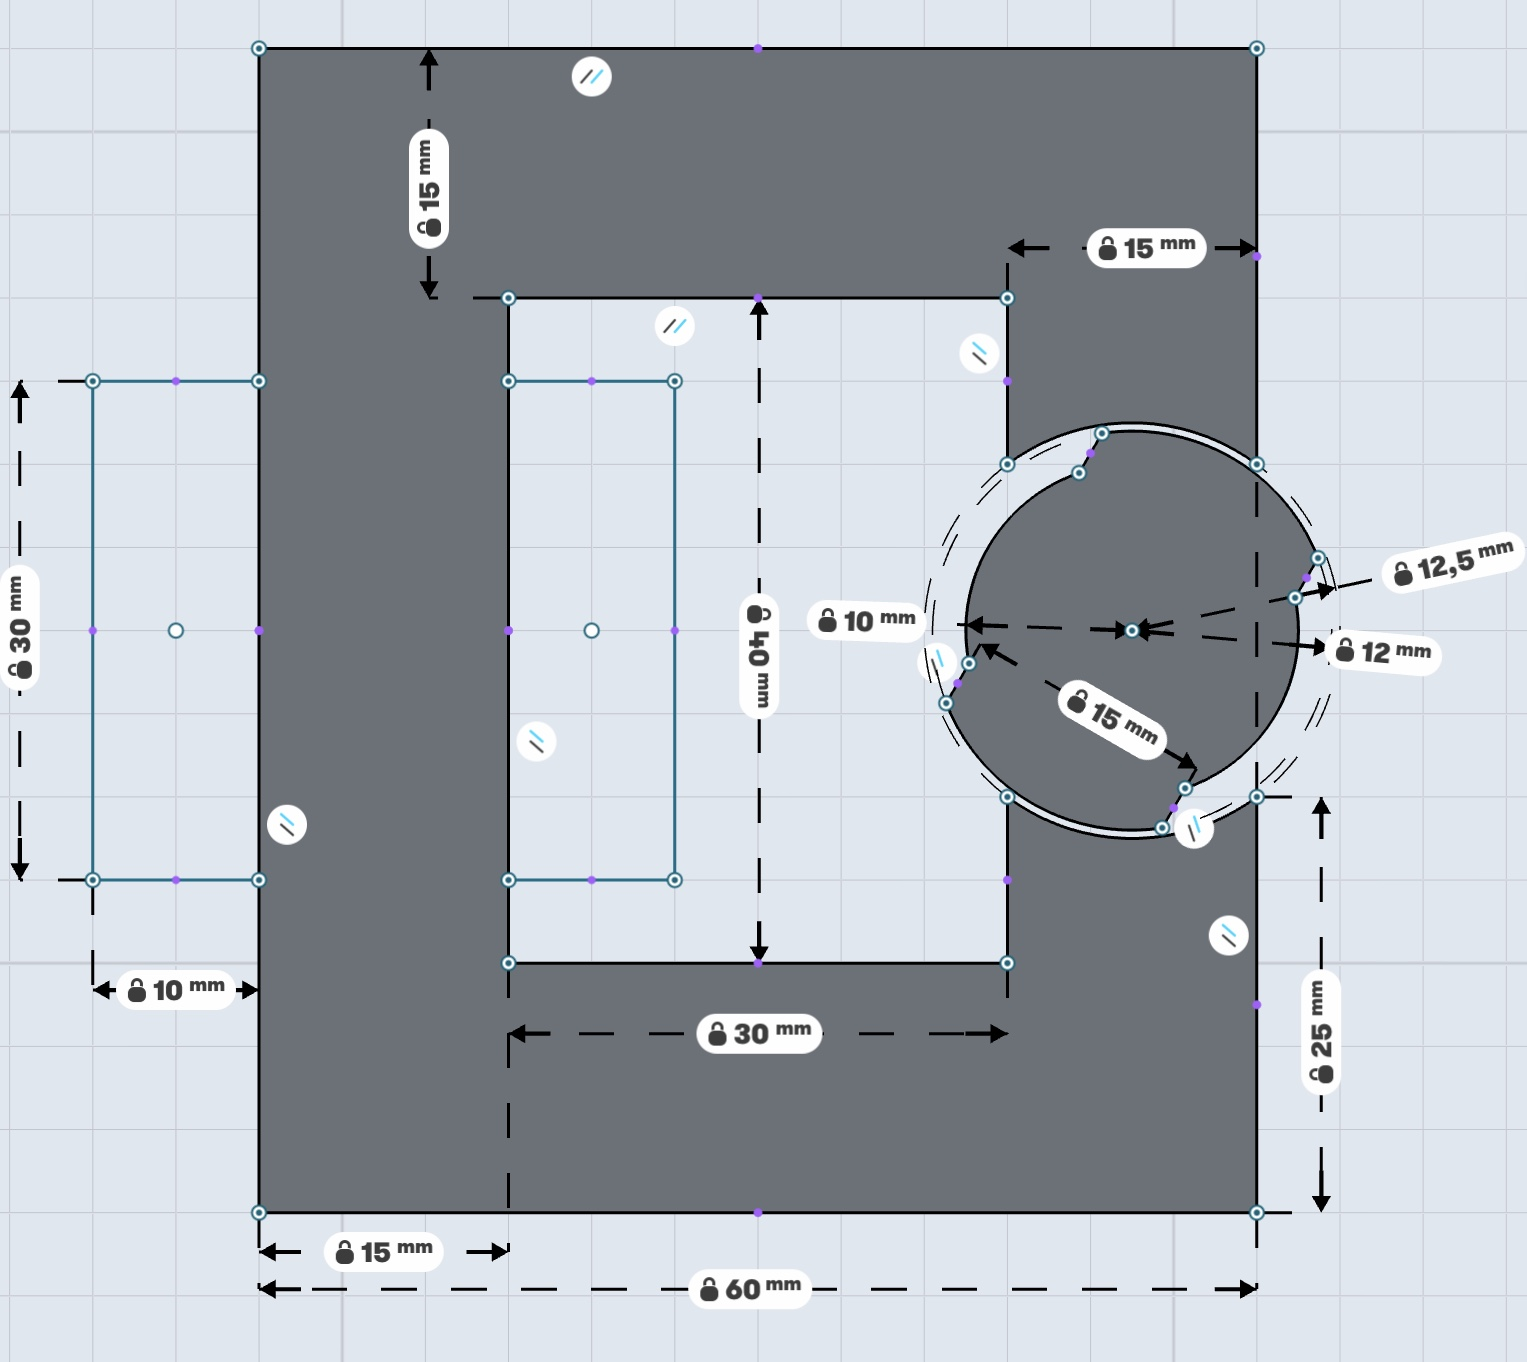
\includegraphics[width=0.5\linewidth]{Figurler/system.jpeg}
	\caption{2D CAD drawing of the variable reluctance machine under investigation.}
	\label{fig:system}
\end{figure}
\section{Analitical Modelling}
In the first subsection analytical modelling of the reluctance and inductance of the system will be made. Then the torque production of the machine will be derived and plotted.


\subsection{Reluctance and Inductance Modeling}
In order to derive an analitical formula for the reluctance and inductance some assumptions are made:
\begin{itemize}
	\item The core is infinitely permeable $\mu_{r}=\infty$,
	\item There is no leakage flux,
	\item The 0 degrees is set as in Fig. \ref{fig:initial}.
	\item The system is linear and hence there is no saturation.
\end{itemize}

\begin{figure}[H]
	\centering
	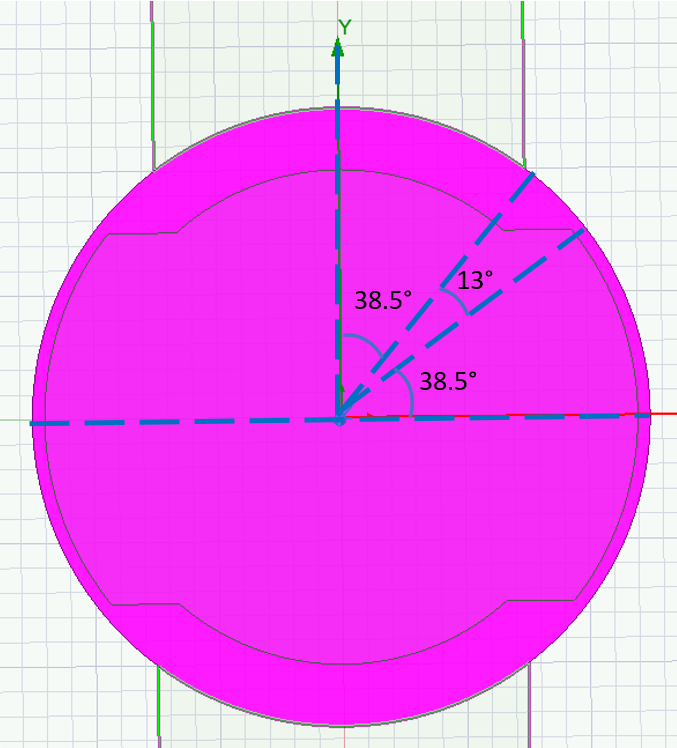
\includegraphics[width=1\linewidth]{E:/Github/EE568/HW1/Rapor/Figurler/initial}
	\caption{Initial rotor position set as $\theta=0 $}degrees
	\label{fig:initial}
\end{figure}
Since the system is assumed to be linear and infinitely permable the reluctance of the machine can be calculated as in (\ref{reluctanceformula}). \enquote{g} is the airgap and equal to 0.5~mm when rotor and the core is fully aligned and maximum 2.5~mm. \enquote{A} is the area between the rotor and the core. Calculation of \enquote{A} is given in (\ref{areaformula}). 
\begin{equation}
R=\frac{2g}{\mu_{0}A}
\label{reluctanceformula}
\end{equation}
\begin{equation}
A=20\frac{\ang{77}2\pi12.5 }{\ang{360}}=335~mm^2
\label{areaformula}
\end{equation}
Then the maximum and minimum reluctance of the machine can be calculated as in(\ref{reluctancecalculation}).
\begin{equation}
\begin{array}{l}
R_{min}=\frac{2g_{max}}{\mu_{0}A}=2.37\times 10^6 \frac{1}{H}\\  
R_{max}=\frac{2g_{min}}{\mu_{0}A}=11.87\times 10^6 \frac{1}{H}
\end{array}
\label{reluctancecalculation}
\end{equation}
At this point it is clear that $R_{min}$ point is achieved when there is a $\ang{90}$ of rotation and $R_{max}$ is achieved when rotation angle \enquote{$\theta$} is 
\ang{-13}$\leq$$\theta$$\leq$\ang{13} and \ang{167}$\leq$$\theta$$\leq$\ang{193}. The piecewise function of reluctance is presented in Table \ref{reluctancetable}.

	\begin{table}[h!]
		\centering
		\caption{Piecewice Function of Reluctance}
		\label{reluctancetable}
		\begin{tabular}{ll}
			\hline
			\ang{0}$\leq$$\theta$$\leq$\ang{13}	& $R=R_{max}$ \\ \hline
			\ang{13}$\leq$$\theta$$\leq$\ang{90}	&  Linear decrease from $R_{max}$ to $R_{min}$ \\ \hline
			\ang{90}$\leq$$\theta$$\leq$\ang{167}	& Linear increase from $R_{min}$ to $R_{max}$\\ \hline
			\ang{167}$\leq$$\theta$$\leq$\ang{180}	& $R=R_{max}$ \\ \hline
		\end{tabular}	
	\end{table}
Ampere law can be stated as in (\ref{amperelaw}) and inductance \enquote{L} can be calculated as in (\ref{inductanceformula}).
\begin{equation}
	NI=\Phi R 
	\label{amperelaw}
\end{equation}
\begin{equation}
L=\frac{\lambda}{I}=A\frac{\Phi}{I}=\frac{N^2}{R}
\label{inductanceformula}
\end{equation}
This equation is valid since $W_{stored}=W^{'}_{stored}$. It was our initial assumption that the system was linear. The maximum inductance($L_{max}$) occurs when there is minimum reluctance and minimum inductance $L_{min}$ occurs when there is maximum reluctance. The inductance of the system can be calculated as in (\ref{inductancecalculation}).

\begin{equation}
\begin{array}{l}
L_{min}=\frac{N^2}{R_{max}}=5.2 mH\\  

L_{max}=\frac{N^2}{R_{min}}=26.5 mH\\  
\end{array}
\label{inductancecalculation}
\end{equation}
Similarly a piecewise function of total inductance is presented in (\ref{inductancetable}).
	\begin{table}[h!]
	\centering
	\caption{Piecewice Function of Total Inductance}
	\label{inductancetable}
	\begin{tabular}{ll}

		\hline
		\ang{0}$\leq$$\theta$$\leq$\ang{13}	& $L=L_{min}$ \\ \hline
		\ang{13}$\leq$$\theta$$\leq$\ang{90}	& Linear increase from $L_{min}$ to $L_{max}$ \\ \hline
		\ang{90}$\leq$$\theta$$\leq$\ang{167}	& Linear decrease from $L_{max}$ to $L_{min}$ \\ \hline
		\ang{167}$\leq$$\theta$$\leq$\ang{180}	& $L=L_{min}$ \\ \hline
	\end{tabular}	
\end{table}
It is important to state that both inductance and reluctance functions are periodic. In Fig. \ref{fig:reluctanceanalitic} and Fig. \ref{fig:inductanceanalitic} a single period of reluctance and inductance are presented respectively.
\begin{figure}[H]
	\centering
	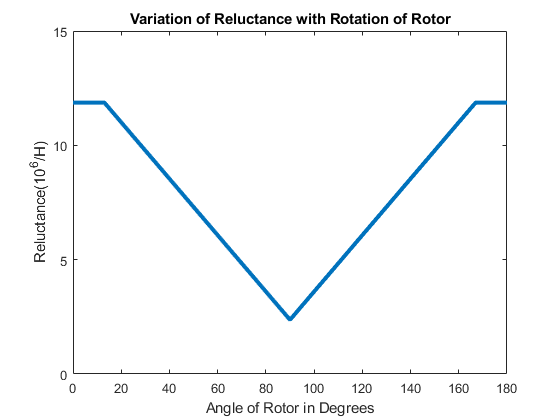
\includegraphics[width=1\linewidth]{E:/Github/EE568/HW1/Rapor/Figurler/reluctance}
	\caption{Variation of Reluctance with Rotation of Rotor}
	\label{fig:reluctanceanalitic}
\end{figure}
\begin{figure}[H]
	\centering
	\includegraphics[width=1\linewidth]{E:/Github/EE568/HW1/Rapor/Figurler/inductance}
	\caption{Variation of Inductance with Rotation of Rotor}
	\label{fig:inductanceanalitic}
\end{figure}

\subsection{Torque Generation}
Since the system is linear $W_{stored}=W^{'}_{stored}=0.5LI^2$. Torque generation can be stated as in (\ref{torqueformula}).

\begin{equation}
T=-\frac{\delta W_{stored}}{\delta\theta}=\frac{\delta W^{'}_{stored}}{\delta\theta}=\frac{\delta(0.5LI^2)}{\delta\theta}=\frac{1}{2}I^2\frac{\delta L}{\delta\theta}=\frac{1}{2}I^2\frac{\Delta L}{\Delta\theta}
\label{torqueformula}
\end{equation}
Hence the piecewise torque generation can be written as in Table \ref{torquetable}. Here it is important to note that all degrees are converted to radians during calculations. Since \enquote{L} increases or decreases linearly the torque generation is constant. The generated torque is presented in Fig. \ref{fig:torqueanalitic}.
	\begin{table}[h!]
	\centering
	\caption{Piecewice Function of Torque Generation}
	\label{torquetable}
	\begin{tabular}{ll}		
		\hline
		\ang{0}$\leq$$\theta$$\leq$\ang{13}	& $T=0 Nm$ \\ \hline
		\ang{13}$\leq$$\theta$$\leq$\ang{90}	& $T=71 Nm$ \\ \hline
		\ang{90}$\leq$$\theta$$\leq$\ang{167}	& $T=-71 Nm$ \\ \hline
		\ang{167}$\leq$$\theta$$\leq$\ang{180}	& $T=0 Nm$ \\ \hline
	\end{tabular}	
\end{table}
\begin{figure}[H]
	\centering
	\includegraphics[width=1\linewidth]{E:/Github/EE568/HW1/Rapor/Figurler/torque}
	\caption{Variation of Torque with Rotation of Rotor}
	\label{fig:torqueanalitic}
\end{figure}

\subsection{Improvements}
The initial assumptions can be modified in order to achieve a better analitic approximation. The first change can be made to core permeability. In reluctance machines laminated steel is often the chosen material for its low cost and low core loss due to reduction of eddy losses. Iron has a relative permeability around 4000. This changes the total reluctance and hence changes the inductance and torque. A second approximation is on the flux path. Similar to current passing from minimum resistance, flux also tends to pass from loops with minimum reluctance. Hence normally the flux path is not distributed homogenously in the core but tends to concentrate close to the inner surface of the core material. 

\section{FEA Modelling(2D- Linear Materials)}
This section consists of three parts. In the first part the flux line distribution of the machine will be presented for \ang{0},\ang{45} and \ang{90} for a linear core material. Then the inductance and the stored energy of the system will be presented. Finally the torque generation for angle variation will be delivered.

\subsection{Flux Line Distibution for \ang{0},\ang{45} and \ang{90}}
The flux line distribution of the rotor for \ang{0},\ang{45} and \ang{90} of rotation are presented in Fig. \ref{fig:5degreeslinear}, \ref{fig:45degreeslinear} and \ref{fig:90degreeslinear} respectively.
\begin{figure}[H]
	\centering
	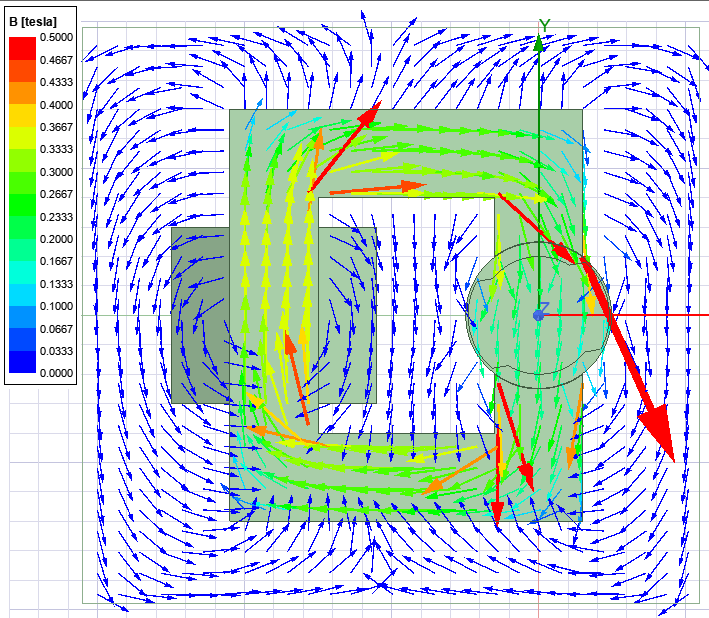
\includegraphics[width=1\linewidth]{E:/Github/EE568/HW1/Rapor/Figurler/Q2/5degrees_linear}
	\caption{Variation of Inductance with Rotation of Rotor}
	\label{fig:5degreeslinear}
\end{figure}

\begin{figure}[H]
	\centering
	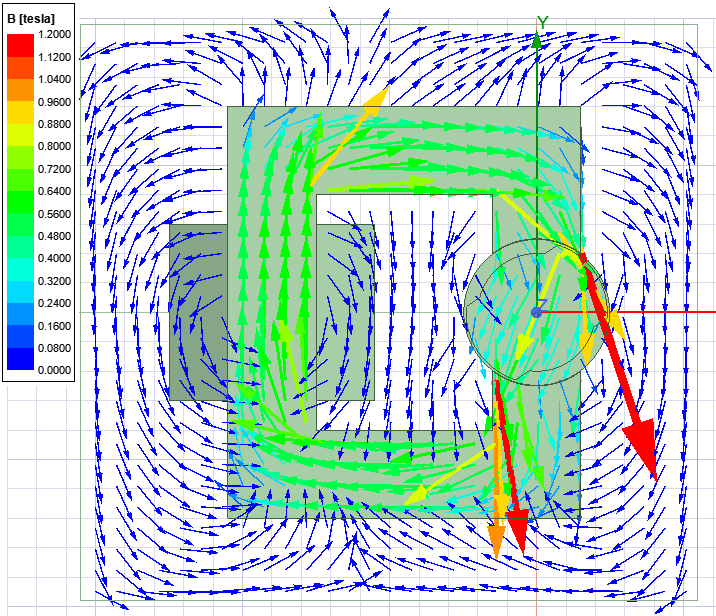
\includegraphics[width=1\linewidth]{Figurler/Q2/45degrees_linear}
	\caption{Flux line distribution for \ang{45} rotation of the rotor.}
	\label{fig:45degreeslinear}
\end{figure}


\begin{figure}[H]
	\centering
	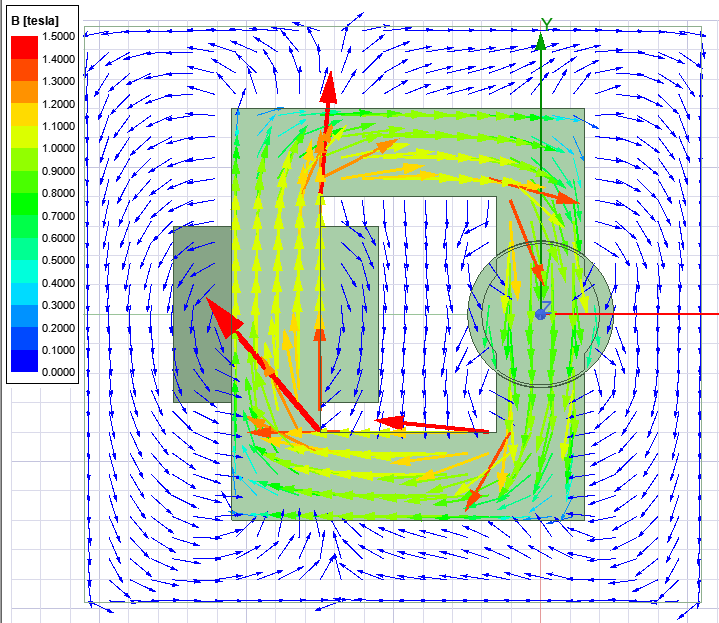
\includegraphics[width=1\linewidth]{Figurler/Q2/90degrees_linear}
	\caption{Flux line distribution for \ang{90} rotation of the rotor.}
	\label{fig:90degreeslinear}
\end{figure}
\subsection{Inductance and Total Stored Energy}
The inductance and the total stored energy calculations are presented in Fig. \ref{fig:degreesinductance} and Fig. \ref{fig:totalenergy} respectively. The total energy are calculated using both BxH and $0.5LI^2$ formulas and for linear systems these two calculations are the expected to be the same. The results in Fig. \ref{fig:totalenergy} clearly proves this hypothesis since there is a perfect overlap in the waveforms.

\begin{figure}[H]
	\centering
	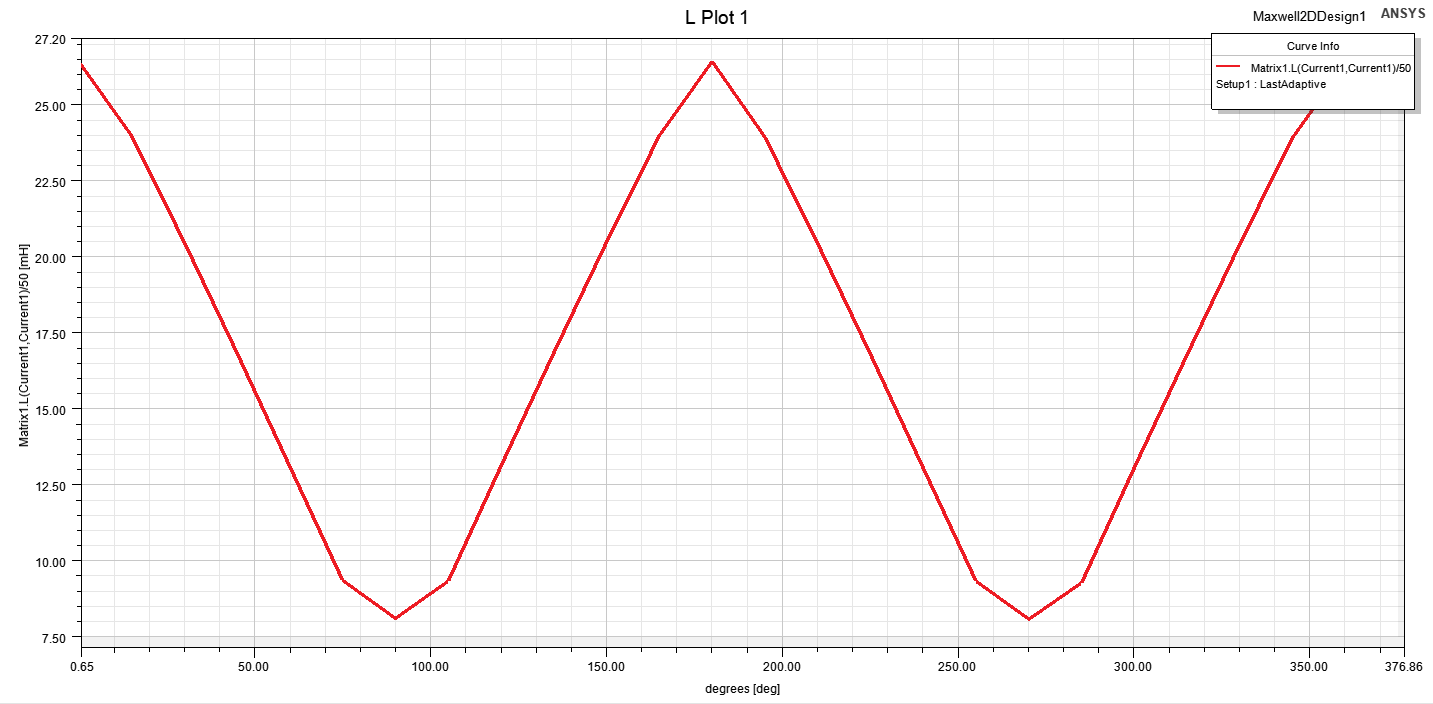
\includegraphics[width=1\linewidth]{Figurler/Q2/degrees_inductance}
	\caption{}
	\label{fig:degreesinductance}
\end{figure}

\begin{figure}[H]
	\centering
	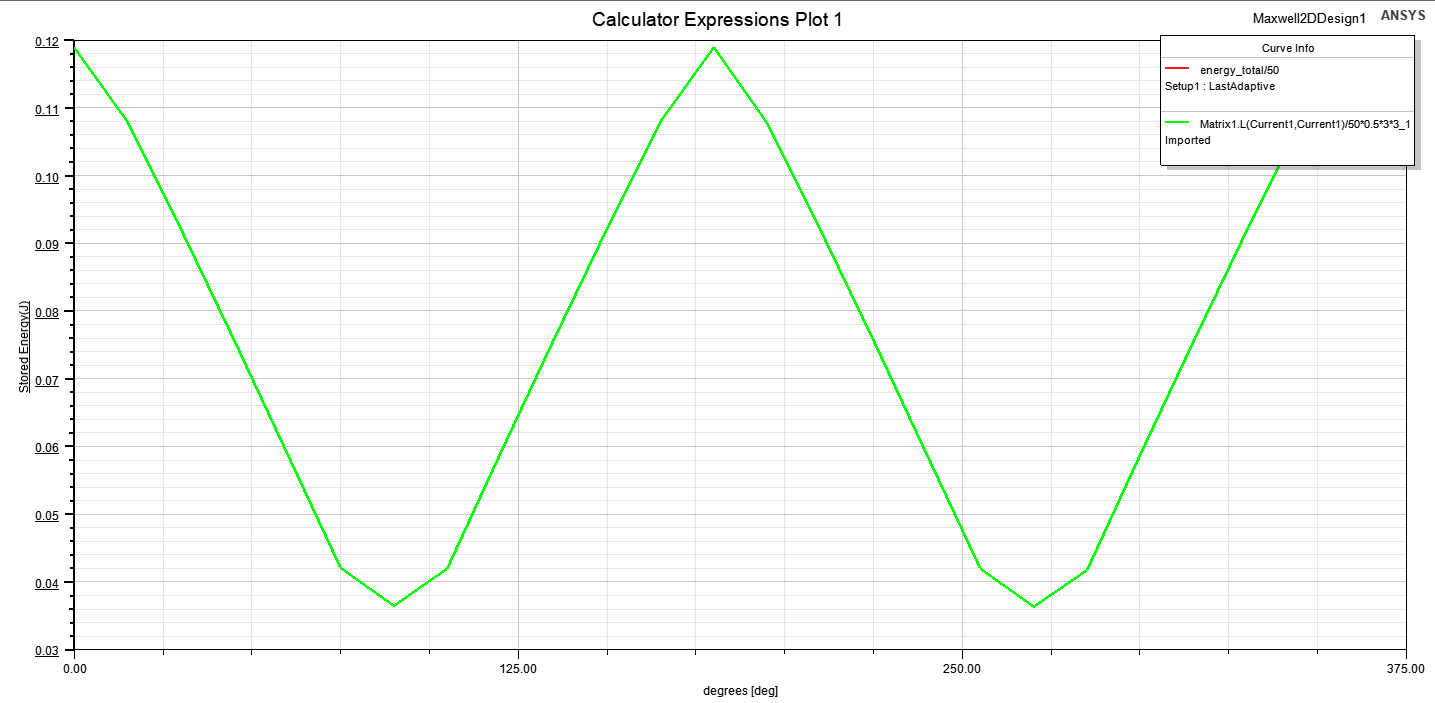
\includegraphics[width=1\linewidth]{Figurler/Q2/total_energy}
	\caption{}
	\label{fig:totalenergy}
\end{figure}

\subsection{Torque Generation}
The torque generation for different rotor angles are presented in Fig. \ref{fig:degreestorque}. The peak points are at 60~Nm. According to our analytical calculations the torque generation should be 71~Nm. The difference is due to fringing and leakage inductance.  
\begin{figure}[H]
	\centering
	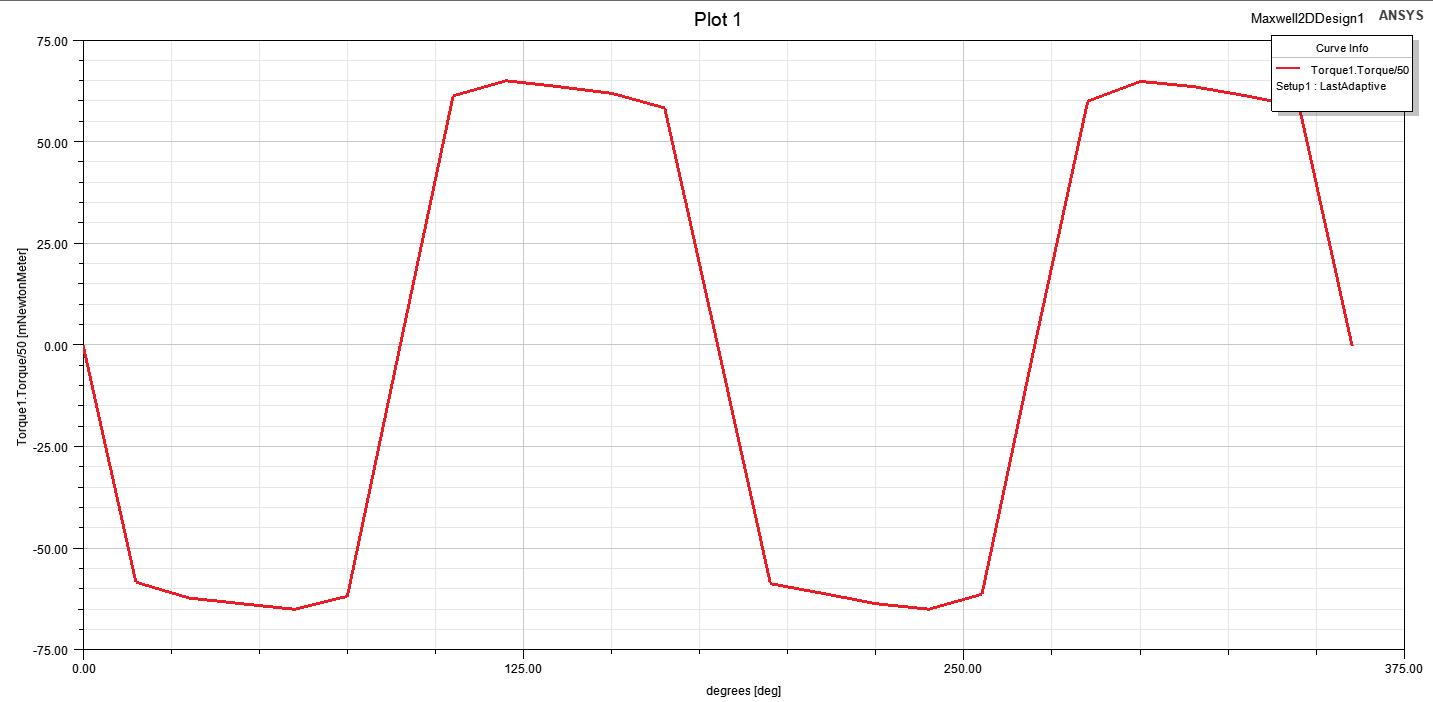
\includegraphics[width=1\linewidth]{Figurler/Q2/degrees_torque}
	\caption{Torque generation for different rotor angles.}
	\label{fig:degreestorque}
\end{figure}


\section{FEA Modelling(2D- Non-Linear Materials)}
In this section the procedure in previous section will be repeated. As for non-linear material ChinaSteel 35CS250H1 was selected. It's B-H curve is presented in Fig. \ref{fig:bh}

\begin{figure}[H]
	\centering
	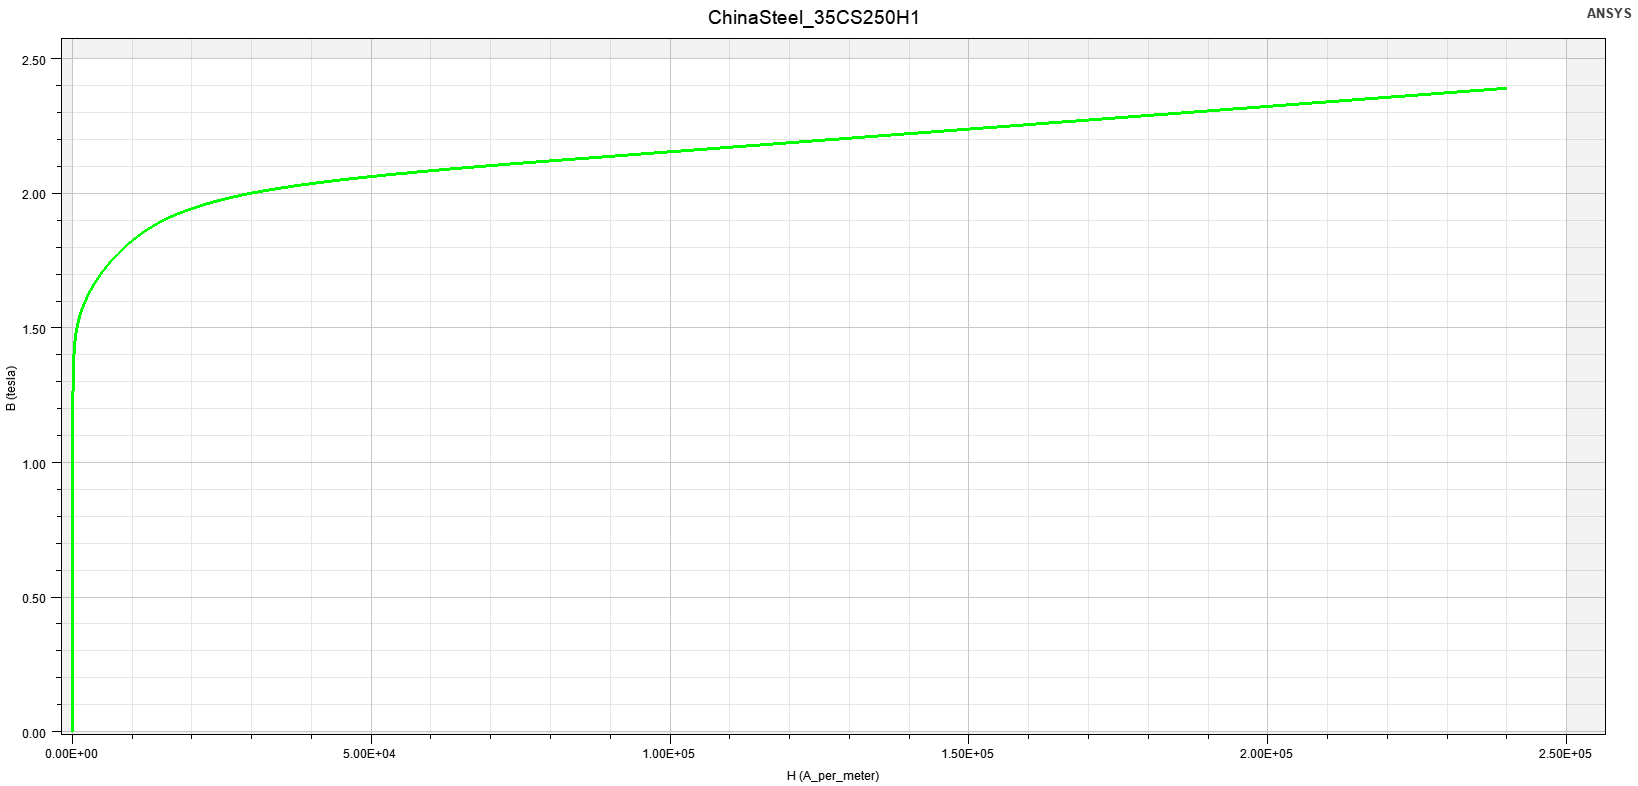
\includegraphics[width=1\linewidth]{Figurler/Q3/B_H}
	\caption{B-H Curve of ChinaSteel 35CS250H1. }
	\label{fig:bh}
\end{figure}

\subsection{Flux Line Distibution for \ang{0},\ang{45} and \ang{90}}
The flux line distribution for \ang{0},\ang{45} and \ang{90} are given in Fig. \ref{fig:zerodeg},\ref{fig:45deg} and \ref{fig:90deg} respectively.

\begin{figure}[H]
	\centering
	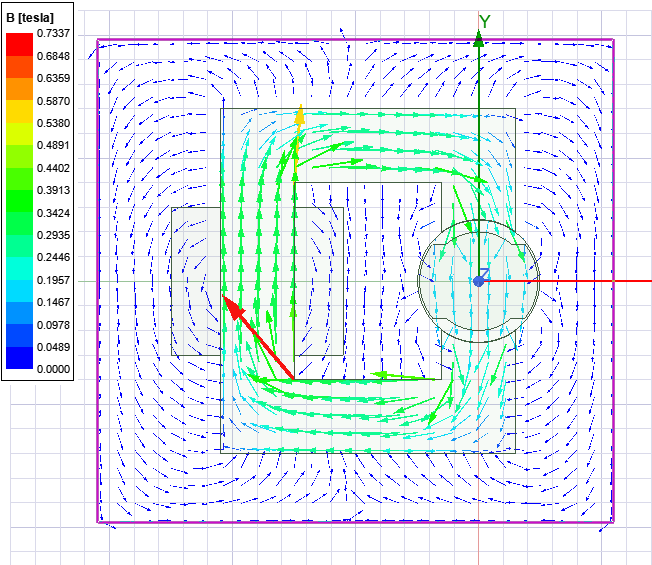
\includegraphics[width=1\linewidth]{Figurler/Q3/zerodeg}
	\caption{Non-linear material zero degrees.}
	\label{fig:zerodeg}
\end{figure}

\begin{figure}[H]
	\centering
	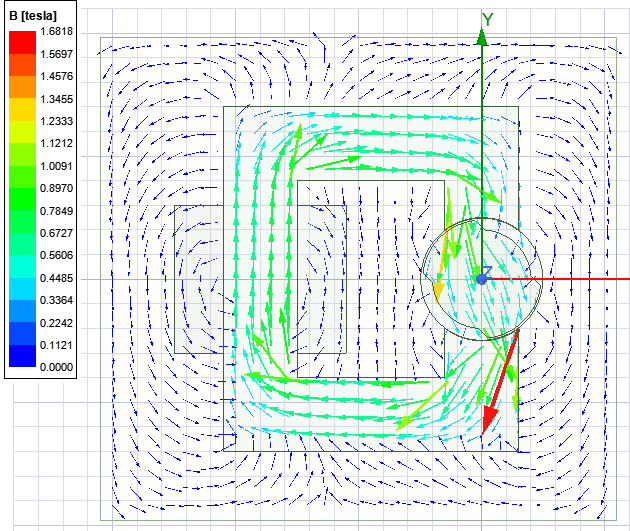
\includegraphics[width=1\linewidth]{Figurler/Q3/45deg}
	\caption{Non-linear material 45 degrees.}
	\label{fig:45deg}
\end{figure}
\begin{figure}[H]
	\centering
	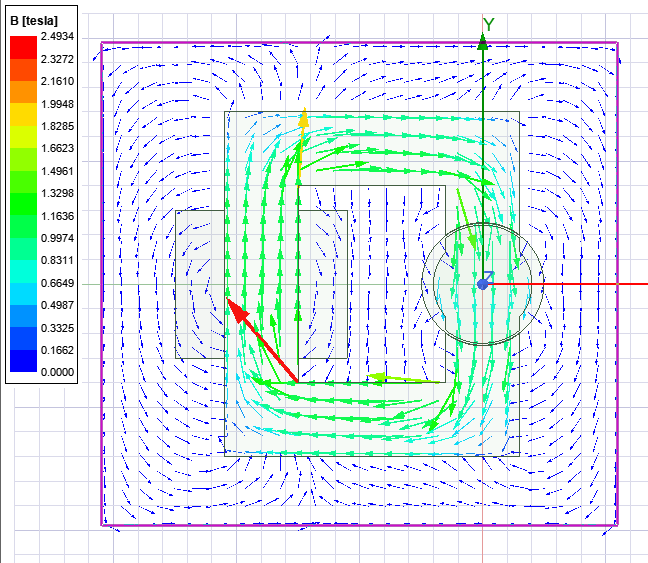
\includegraphics[width=1\linewidth]{Figurler/Q3/90deg}
	\caption{Non-linear material 90 degrees.}
	\label{fig:90deg}
\end{figure}


\subsection{Inductance and Total Stored Energy}
The inductance and system energy variation vs rotor angle are given in Fig. \ref{fig:inductance_nonlinear} and \ref{fig:storedenergy1} respectively. Since the system is non-linear the energy and the co-energy are the system are not equal to each other. Since $0.5LI^2$ gives us the co-energy the waveforms are different than eachother.
\begin{figure}[H]
	\centering
	\includegraphics[width=1\linewidth]{Figurler/Q3/inductance}
	\caption{Variation of inductance vs rotor angle.}
	\label{fig:inductance_nonlinear}
\end{figure}

\begin{figure}[H]
	\centering
	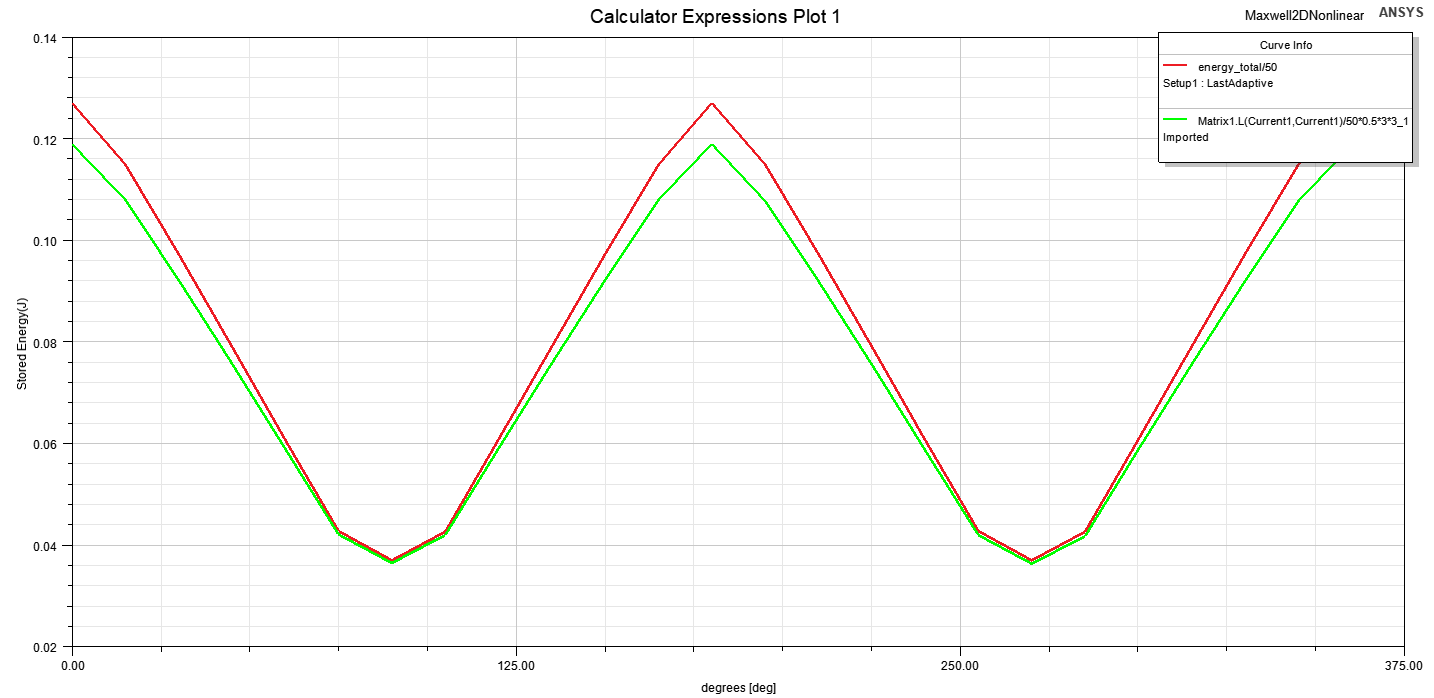
\includegraphics[width=1\linewidth]{Figurler/Q3/stored_energy}
	\caption{Total stored energy.}
	\label{fig:storedenergy1}
\end{figure}


\subsection{Torque Generation}
The torque generation of the system with non-linear core material is presented in Fig. \ref{fig:torquenonlinear}.
\begin{figure}[H]
	\centering
	\includegraphics[width=1\linewidth]{Figurler/Q3/torque}
	\caption{Torque generation}
	\label{fig:torquenonlinear}
\end{figure}

\section{Control Method}
From Q2 and Q3 it is clear that the machine generated positive torque between zero to 90 degrees. Then the machine generates torque in the opposite direction between 90 to 180 degrees. However, this is valid for constant DC excitation. With a DC excitation it is not possible to generate rotation motion. If constant stator current is applied the rotor will oscillate and will try to align itself with the core where it has minimum reluctance.\\
To generated a rotation motion the direction of the current can be altered. By applying negative current the direction of the torque changes. Hence by applying a square wave a positive torque can be generated. In order to show proof of concept, the direction of applied current was reversed. The generated negative torque is presented in Fig. \ref{fig:negativetorque}. Assuming that current direction can be changed at $T=0Nm$ points the torque in Fig. \ref{fig:abstorque} can be generated.

\begin{figure}[H]
	\centering
	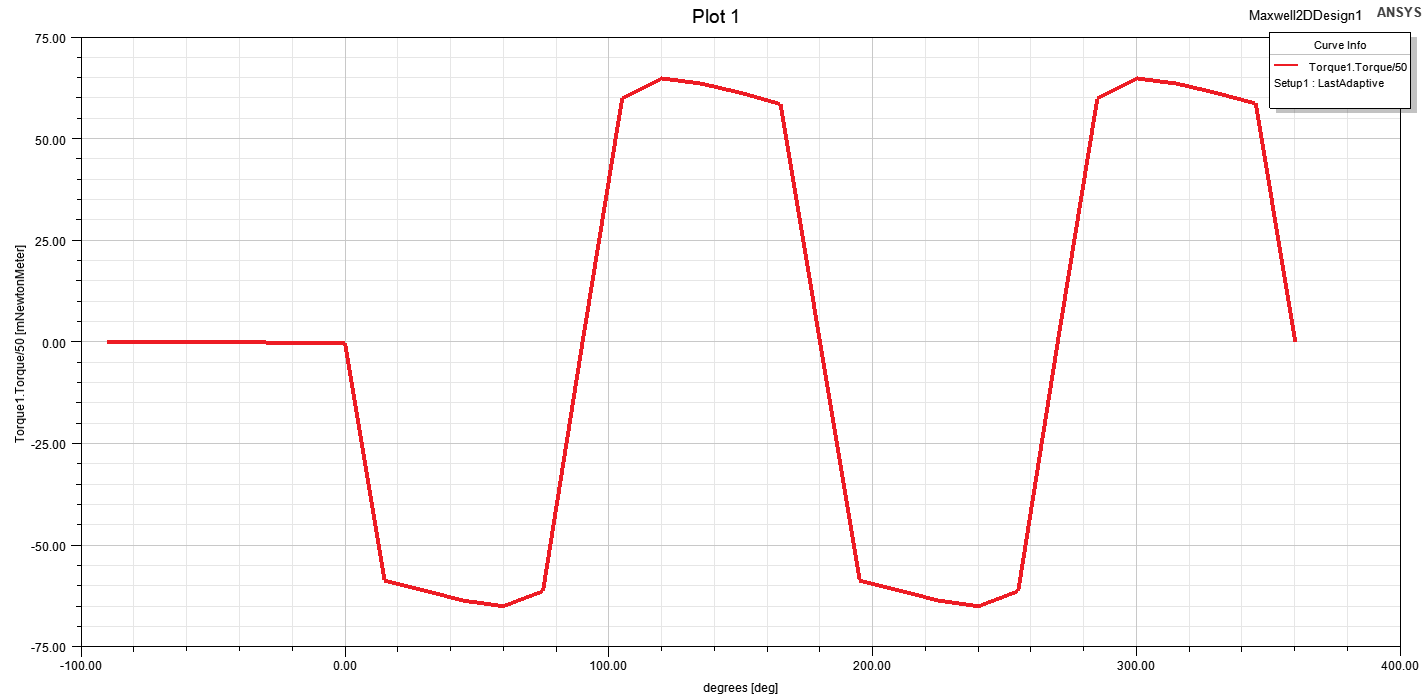
\includegraphics[width=1\linewidth]{Figurler/Q4/negative_torque}
	\caption{Torque generation for reverse polarity current.}
	\label{fig:negativetorque}
\end{figure}

\begin{figure}[H]
	\centering
	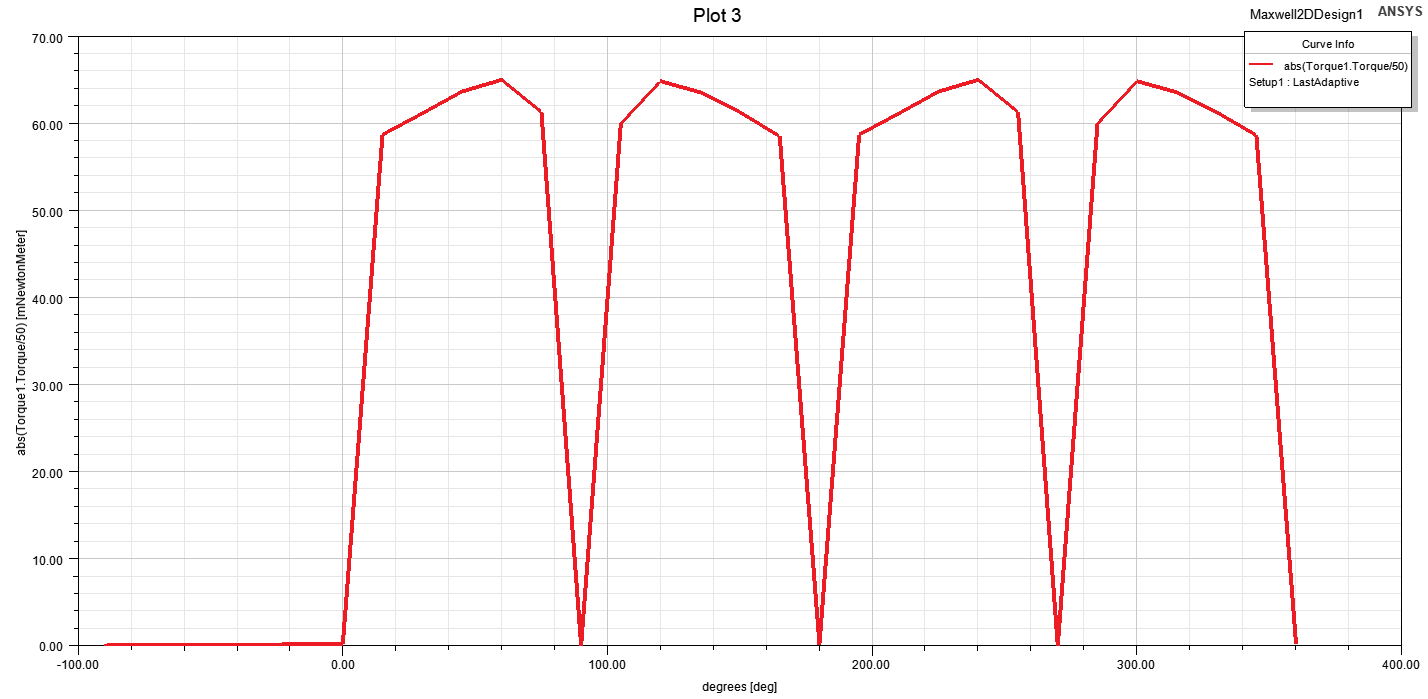
\includegraphics[width=1\linewidth]{Figurler/Q4/abstorque}
	\caption{Torque generated using proposed control method.}
	\label{fig:abstorque}
\end{figure}

\section{Bonus: Motion Animation}
The motion animation can be found on Github repository.

\section{Conclusion}

In this report, fundamental concepts governing variable reluctance machines were observed. The effects of neglecting fringing flux and saturation on the analytical derivation of reluctance, inductance and torque were analyzed. In linear case where the rotor and the stator are fully aligned, the maximum flux density in the core was about 1.5~T. Therefore changing the material from linear to non-linear didnot present significant changes due to the fact that selected material has a high saturation point arond 1.7~T. The analytically calculated inductances and the results overlaps with 10\% error due to neglecting core material permeability and the fringing flux. The analitically calculated torque was 71~Nm and the peak torque found in 2D linear magnetostatic solution is 68~Nm which results in 4\% error.

\end{document}
